En esta sección se detallarán los casos de uso pertenecientes al subsistema de datos. La figura \ref{fig:casos_uso_subsistema_datos} muestra el diagrama de casos de uso de dicho subsistema.

\begin{figure}[h]
\centering
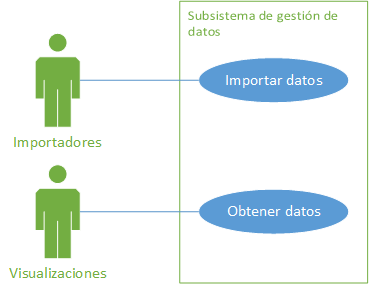
\includegraphics{casos_uso_datos}
\caption{Diagrama de casos de uso del subsistema de datos}
\label{fig:casos_uso_subsistema_datos}
\end{figure}

\subsubsection{Caso de uso ``importar datos''}
\begin{description}
\item[Descripción] Un importador quiere incluir nueva información en el sistema.
\item[Actores] Un importador.
\item[Escenario principal] \hfill
							\begin{enumerate}
							\item El importador envía una petición POST al subsistema de datos incluyendo un fichero XML conforme a un XML Schema definido y con los datos a incluir en el sistema.
							\item El subsistema de datos comprueba si la dirección de origen de la petición está en la lista blanca.
							\item El subsistema de datos procesa la petición convirtiendo la información del fichero XML a un modelo propio.
							\item El subsistema de datos persiste en la base de datos el modelo creado anteriormente.
							\item El subsistema envía una respuesta 200 (\textit{OK}) al importador.
							\end{enumerate}
\item[Escenario alternativo 1] Los datos enviados por el importador no se ajustan al XML Schema.
							\begin{enumerate}
							\item El subsistema de datos no insertará ningún dato en la base de datos.
							\item El subsistema de datos envía una respuesta de error al importador.
							\end{enumerate}
\item[Escenario alternativo 2] El verbo utilizado por el importador no es el correcto (GET, PUT, etc).
							\begin{enumerate}
							\item El subsistema de datos no insertará ningún dato en la base de datos.
							\item El subsistema de datos envía una respuesta de error 405 (\textit{Method not Allowed}) al importador.
							\end{enumerate}
\item[Escenario alternativo 3] La petición realizada por el importador no incluye el fichero XML con los datos.
							\begin{enumerate}
							\item El subsistema de datos no insertará ningún dato en la base de datos.
							\item El subsistema de datos envía una respuesta de error 400 (\textit{Bad Request}) al importador.
							\end{enumerate}
\item[Escenario alternativo 4] La petición proviene de un origen no confiable
							\begin{enumerate}
							\item El subsistema de datos aborta la petición con un código de error 403 (\textit{Forbidden}).
							\end{enumerate}
\end{description}	

\subsubsection{Caso de uso ``obtener datos''}
\begin{description}
\item[Descripción] Una visualización pide datos para presentarlos al usuario de forma atractiva.
\item[Actores] Visualizaciones.
\item[Escenario principal] 	\hfill
							\begin{enumerate}
							\item La visualización lanza una petición GET al subsistema de datos.
							\item El subsistema de datos devuelve un fichero JSON con los datos correspondientes a la petición realizada.
							\item La visualización procesa los datos recibidos para presentarlos de forma visual.
							\end{enumerate}
\item[Escenario alternativo 1] La petición de la visualización es errónea.
							\begin{enumerate}
							\item La visualización lanza una petición al subsistema de datos.
							\item El subsistema de datos responde con un código de error HTTP.
							\end{enumerate}
\end{description}